\chapter{Sinesweep analysis}\label{chap:sinesweep}
The inputs provided are two sine sweep equal signal with different sample
frequencies \(5\) \si{\milli\second} and \(10\) \si{\milli\second} rispectively.
To visualize the spectra of the signals, by \emph{fft} is performed on both the
signal.
\begin{figure}[htb]
	\centering
	\subfloat[][\emph{slow}]
		{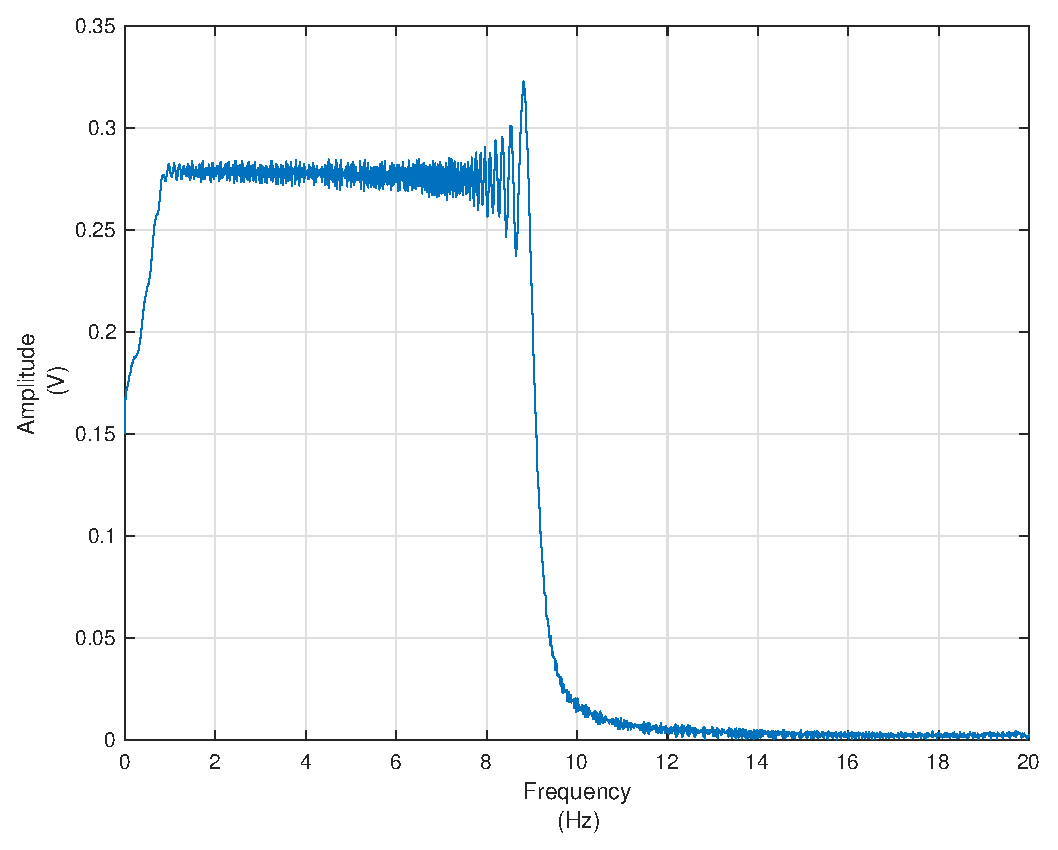
\includegraphics[width=0.45\textwidth]{Fouriertrasformslow}}	\,
	\subfloat[][\emph{fast}]
		{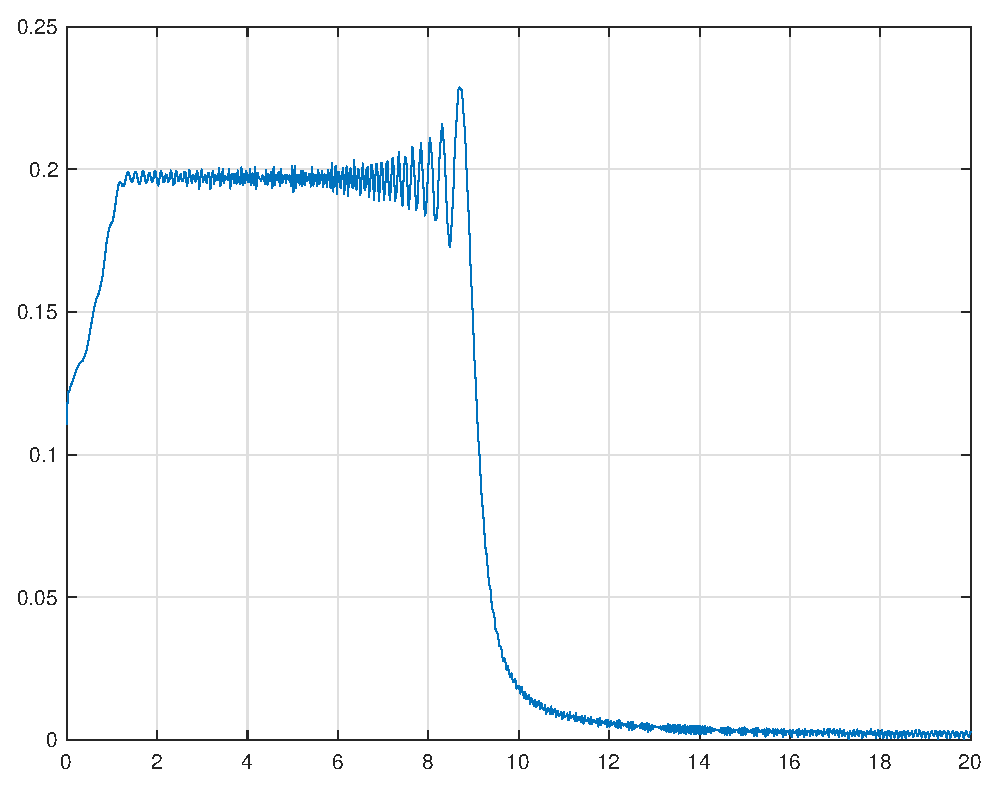
\includegraphics[width=0.45\textwidth]{Fouriertrasformfast}}
	\caption{Sine sweep spectrum}
	\label{fig:spectral}
\end{figure}
The spectrum is plotted with the real frequencies in figure \ref{fig:spectral}.\\
Although the two signals sweep the same frequency range and the difference is
only in the sampling time. These include the resonance peaks of the transfer
function.
On the other hand, the spectrum of the sinusoidal scan excites each frequency
for a limited period of time so it is possible to notice that the third mode is
not clearly visible.
\begin{figure}[htb]
	\centering
	\subfloat[][Respect mass 1]
		{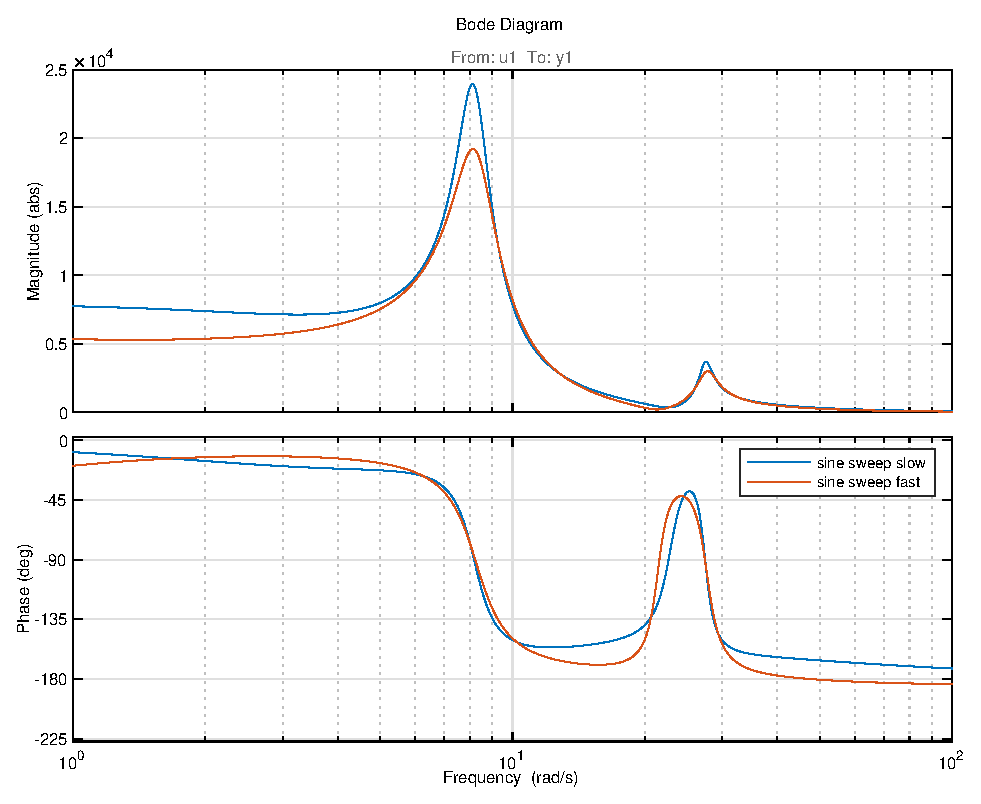
\includegraphics[width=0.5\textwidth]{sinecomparebodediagram1}}	\\
	\subfloat[][Respect mass 2]
		{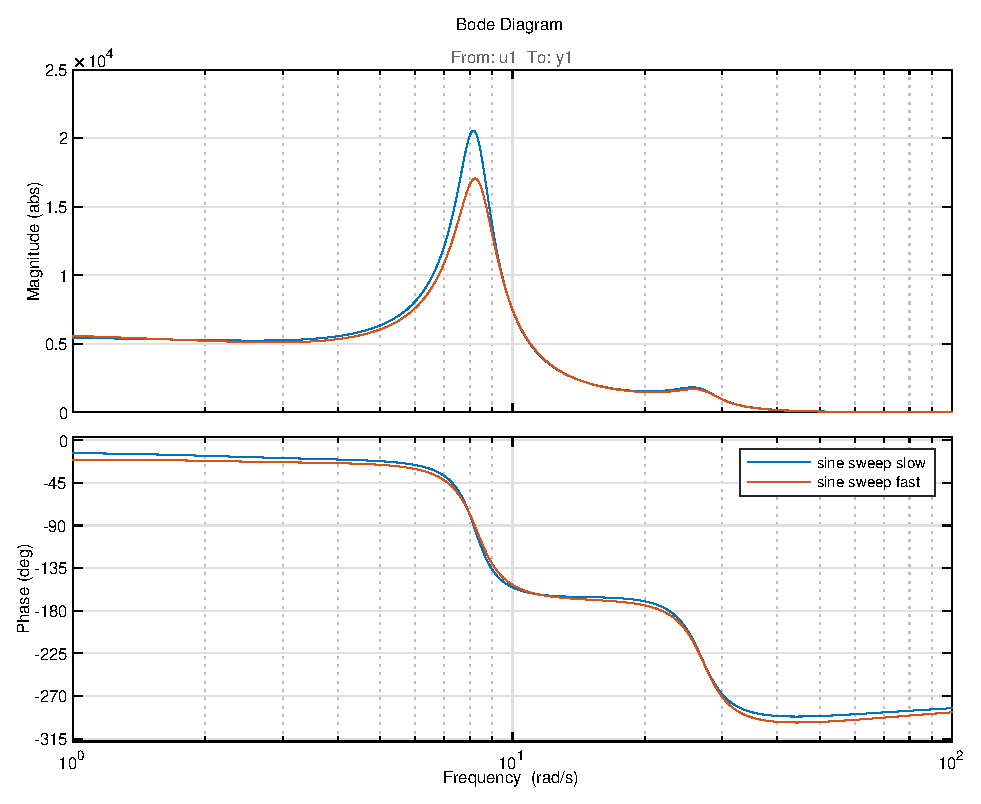
\includegraphics[width=0.5\textwidth]{sinecomparebodediagram2}}	\\
	\subfloat[][Respect mass 3]
		{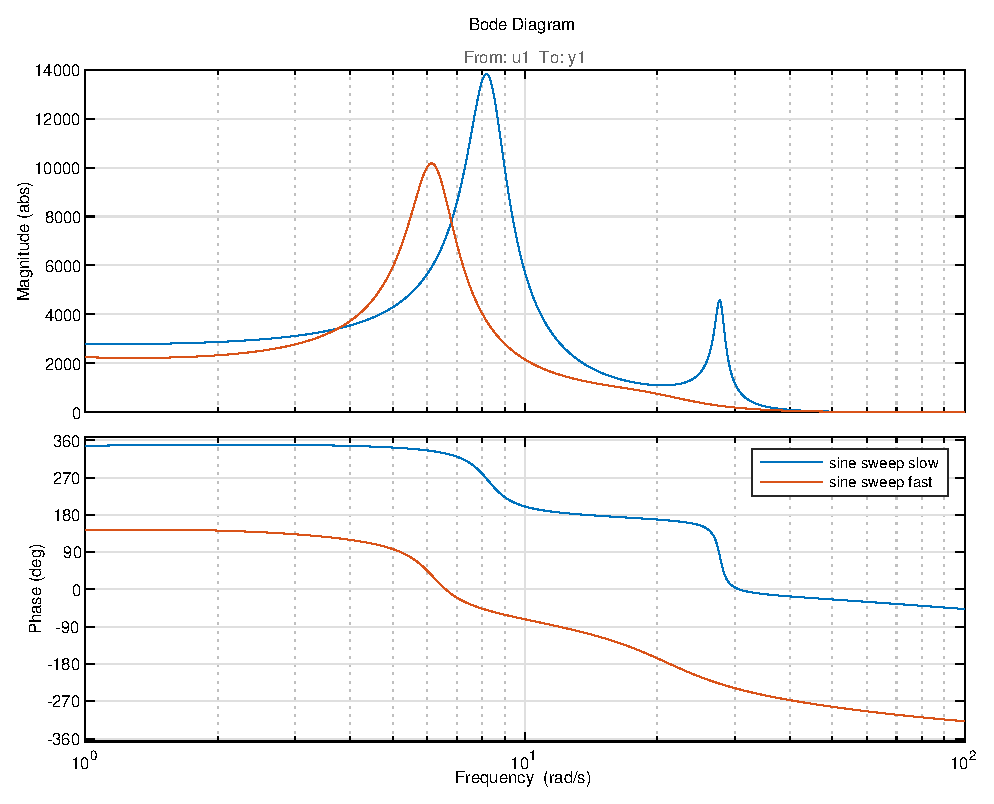
\includegraphics[width=0.5\textwidth]{sinecomparebodediagram3}}	\\
	\caption{Comparison sine sweep outputs of the system}
	\label{fig:bodesinesweep}
\end{figure}
